%%%%%%%%%%%%%%%%%%%%%%%%%%%%%%%%%%%%%%%%%
% Beamer Presentation
% LaTeX Template
% Version 1.0 (10/11/12)
%
% This template has been downloaded from:
% http://www.LaTeXTemplates.com
%
% License:
% CC BY-NC-SA 3.0 (http://creativecommons.org/licenses/by-nc-sa/3.0/)
%
%%%%%%%%%%%%%%%%%%%%%%%%%%%%%%%%%%%%%%%%%

%----------------------------------------------------------------------------------------
%	PACKAGES AND THEMES
%----------------------------------------------------------------------------------------

\documentclass{beamer}

\mode<presentation> {

% The Beamer class comes with a number of default slide themes
% which change the colors and layouts of slides. Below this is a list
% of all the themes, uncomment each in turn to see what they look like.

%\usetheme{default}
%\usetheme{AnnArbor}
%\usetheme{Antibes}
%\usetheme{Bergen}
%\usetheme{Berkeley}
%\usetheme{Berlin}
%\usetheme{Boadilla}
%\usetheme{CambridgeUS}
%\usetheme{Copenhagen}
%\usetheme{Darmstadt}
%\usetheme{Dresden}
%\usetheme{Frankfurt}
%\usetheme{Goettingen}
%\usetheme{Hannover}
%\usetheme{Ilmenau}
%\usetheme{JuanLesPins}
%\usetheme{Luebeck}
%\usetheme{Madrid}
%\usetheme{Malmoe}
%\usetheme{Marburg}
%\usetheme{Montpellier}
%\usetheme{PaloAlto}
%\usetheme{Pittsburgh}
%\usetheme{Rochester}
%\usetheme{Singapore}
%\usetheme{Szeged}
\usetheme{Warsaw}

% As well as themes, the Beamer class has a number of color themes
% for any slide theme. Uncomment each of these in turn to see how it
% changes the colors of your current slide theme.

%\usecolortheme{albatross}
%\usecolortheme{beaver}
%\usecolortheme{beetle}
%\usecolortheme{crane}
%\usecolortheme{dolphin}
%\usecolortheme{dove}
%\usecolortheme{fly}
%\usecolortheme{lily}
%\usecolortheme{orchid}
%\usecolortheme{rose}
%\usecolortheme{seagull}
%\usecolortheme{seahorse}
%\usecolortheme{whale}
%\usecolortheme{wolverine}

%\setbeamertemplate{footline} % To remove the footer line in all slides uncomment this line
%\setbeamertemplate{footline}[page number] % To replace the footer line in all slides with a simple slide count uncomment this line

%\setbeamertemplate{navigation symbols}{} % To remove the navigation symbols from the bottom of all slides uncomment this line
}

\usepackage{graphicx} % Allows including images
\usepackage{booktabs} % Allows the use of \toprule, \midrule and \bottomrule in tables
\usepackage{xcolor}
\usepackage{tikz}
\usepackage[tikz]{bclogo}
\usepackage[absolute,overlay]{textpos}
\usepackage{tcolorbox}
\usepackage{makecell}
\usepackage{multirow}

\newcommand{\imp}[1]{{\color{red}{#1}}}
\newcommand{\remark}[1]{{\color{blue}{#1}}}
\newcommand{\atten}[1]{{\color{green}{#1}}}
\newcommand\Fontvi{\fontsize{9}{10.2}\selectfont}

\newcommand{\tfidf}{\emph{tf-idf}}
\newcommand{\NMF}{\emph{NMF}}

\definecolor{mygreen}{rgb}{0, 0.5, 0}
\newcommand{\PA}[1]{{\color{mygreen}{#1}}}

\usepackage[utf8]{inputenc}

%----------------------------------------------------------------------------------------
%	TITLE PAGE
%----------------------------------------------------------------------------------------

\title[CRIStAL]{Concours Maître de Conférences\\ CRIStAL} % The short title appears at the bottom of every slide, the full title is only on the title page

\author{Pegah ALIZADEH} % Your name
\institute[GREYC] % Your institution as it will appear on the bottom of every slide, may be shorthand to save space
{Université de Caen Normandie (GREYC) \\ 
\includegraphics[scale=0.08]{images/greyc} \\ % Your institution for the title page
\medskip
\textit{pegah.alizadeh@unicaen.fr} % Your email address
}
\date{22 May 2018} % Date, can be changed to a custom date

\begin{document}


\begin{frame}
\titlepage % Print the title page as the first slide
\end{frame}

%\begin{frame}{Outline}
%\tableofcontents
%\end{frame}



%----------------------------------------------------------------------------------------
%	PRESENTATION SLIDES
%----------------------------------------------------------------------------------------
\setbeamercolor{background canvas}{bg=blue!20}
\begin{frame}
	\begin{center}
	\textbf{Parcours Professionnel et Académique}
	\end{center}
\end{frame}
{\setbeamercolor{background canvas}{bg=white}
%------------------------------------------------

\begin{frame}{Formation et Expérience Professionnelle Avant la Thèse}

\begin{block}{Formation}
	\textbf{2001 - 2005} : Licence en Mathématique.\\
	Université Shahid Beheshti (Téhéran, Iran).\\
	\textbf{2006 - 2008} : Master en Mathématique. \\
	Université international d’Imam Khomeini (Qazvin-Iran).
\end{block}
%%%%
\begin{block}{Expérience Professionnelle}
\textbf{2008-2009}: Programmatrice et conceptrice de BDD.\\
Entreprise Soroush Ray Pardazan ( Karaj, Iran ).\\
\textbf{2010 - 2011}: Enseignante de Mathématiques. \\
Université de Payam Nur de Karaj et Université Azad de Karaj, Iran
\end{block}

\end{frame}
%-------------------------------------------------

\begin{frame}{Formation et Expérience Professionnelle}

\begin{block}{Formation}
\textbf{Février - Mai 2012}: Stage de recherche en génie logiciel.\\
Université libre de Bolzano ( Bolzano, Italie )\\
\textbf{2012-2016}: Doctorat en Informatique.\\
LIPN, Université Paris 13.
\end{block}

\begin{block}{Expérience Professionnelle}
\textbf{2015-2016, 2016-2017}: ATER.\\
LIPN, Université Paris 13. Université Paris Dauphine.\\
\textbf{2017-2018}: Post-Doctorante en Machine Learning - Traitement Automatique de Langues.\\
GREYC, Université de Caen, Normandie. 
\end{block}

\end{frame}
%------------------------------------------------
\begin{frame}{Thèse}

\begin{itemize} 
\item \textbf{Dates}: Octobre 2012 - Décembre 2016
\item \textbf{Lieu}: Laboratoire d’Informatique de Paris Nord (LIPN),
Université Paris 13.
\item \textbf{Intitulé}: Élicitation et planification dans les processus de
décision de Markov avec des récompenses inconnues.
\item \textbf{Directeur de thèse}: Yann Chevaleyre.
\item \textbf{Rapporteurs} : Nicolas MAUDET (Université Pierre et
Marie Curie), Bruno ZANUTTINI (Université de Caen).
\item \textbf{Jury}: Yann CHEVALEYRE, Jérôme LANG, Nicolas
MAUDET, Henry SOLDANO, Paolo VIAPPIANI, Bruno
ZANUTTINI
\end{itemize}
	
\end{frame}
%------------------------------------------------

\setbeamercolor{background canvas}{bg=blue!20}
\begin{frame}
	\begin{center}
	\textbf{Thèmes de Recherche}
	\end{center}
\end{frame}
{\setbeamercolor{background canvas}{bg=white}


\begin{frame}{Thémes de recherche et applications}

\begin{picture}(320,250)

%%%%%%%%%%%%%%%%%%%%%%%%%%%%%%%%%%%%%
\put(-20,250){
\begin{minipage}[t]{0.56\linewidth}
{
\begin{block}{Apprentissage par Renforcement}
Processus de décision markov (MDP)
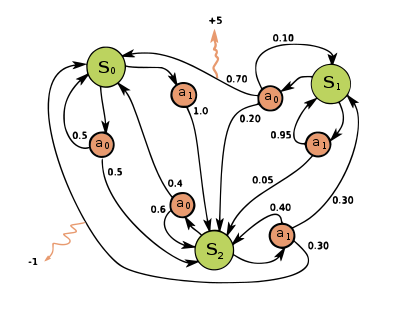
\includegraphics[height=2.25cm]{./images/Themes_MDP.png}
\end{block}
}
\end{minipage}
}

%\put(0,130){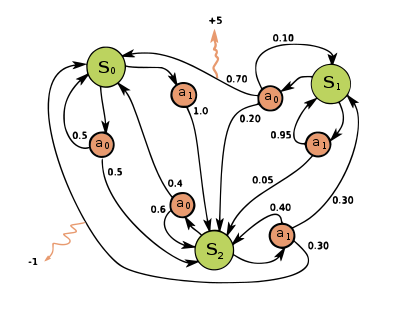
\includegraphics[height=3.0cm]{./images/Themes_MDP.png}}
%%%%%%%%%%%%%%%%%%%%%%%%%%%%%%%%%%%%%


%%%%%%%%%%%%%%%%%%%%%%%%%%%%%%%%%%%%%
\put(-20,140){
\begin{minipage}[t]{0.56\linewidth}
{
\begin{block}{Traitement Automatique de Langages}
Clustering et Neural networks \\
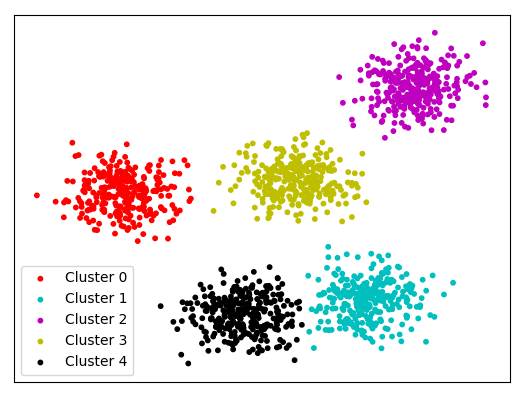
\includegraphics[height=2.0cm]{./images/Themes_Clustering.png}
%\item \\
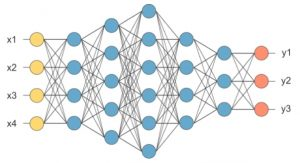
\includegraphics[height=1.7cm]{./images/Themes_DNN.jpg}\end{block}
}
\end{minipage}
}

%\put(0,20){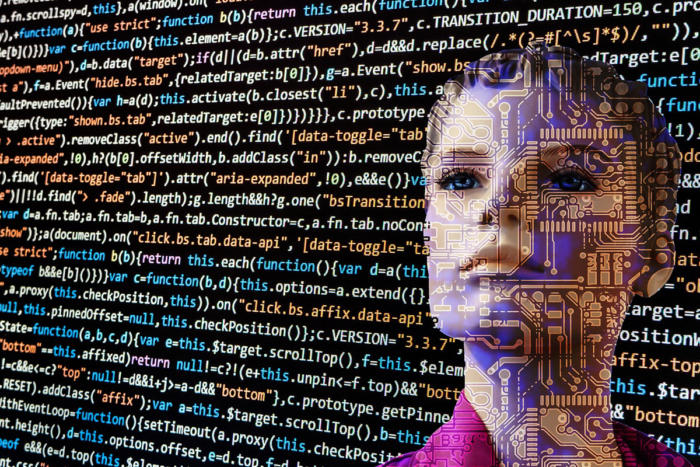
\includegraphics[height=2.5cm]{./images/Themes_NLP.jpg}}
%%%%%%%%%%%%%%%%%%%%%%%%%%%%%%%%%%%%%

%%%%%%%%%%%%%%%%%%%%%%%%%%%%%%%%%%%%%
\put(150,250){ \begin{minipage}[t]{0.75\linewidth}
{ \begin{itemize} \item Optimal Planning \end{itemize} }
\end{minipage} }

\put(170,190){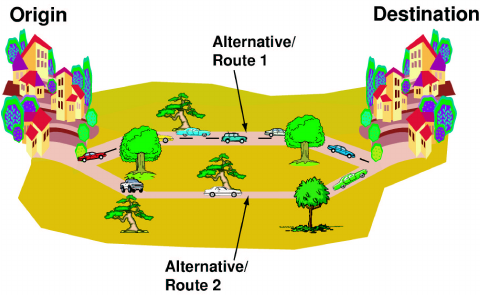
\includegraphics[height=1.75cm]{./images/Themes_routes.png}}
%%%%%%%%%%%%%%%%%%%%%%%%%%%%%%%%%%%%%

%%%%%%%%%%%%%%%%%%%%%%%%%%%%%%%%%%%%%
\put(220,205){ \begin{minipage}[t]{0.75\linewidth}
{ \begin{itemize} \item Internet of Things \end{itemize} }
\end{minipage} }

\put(255,145){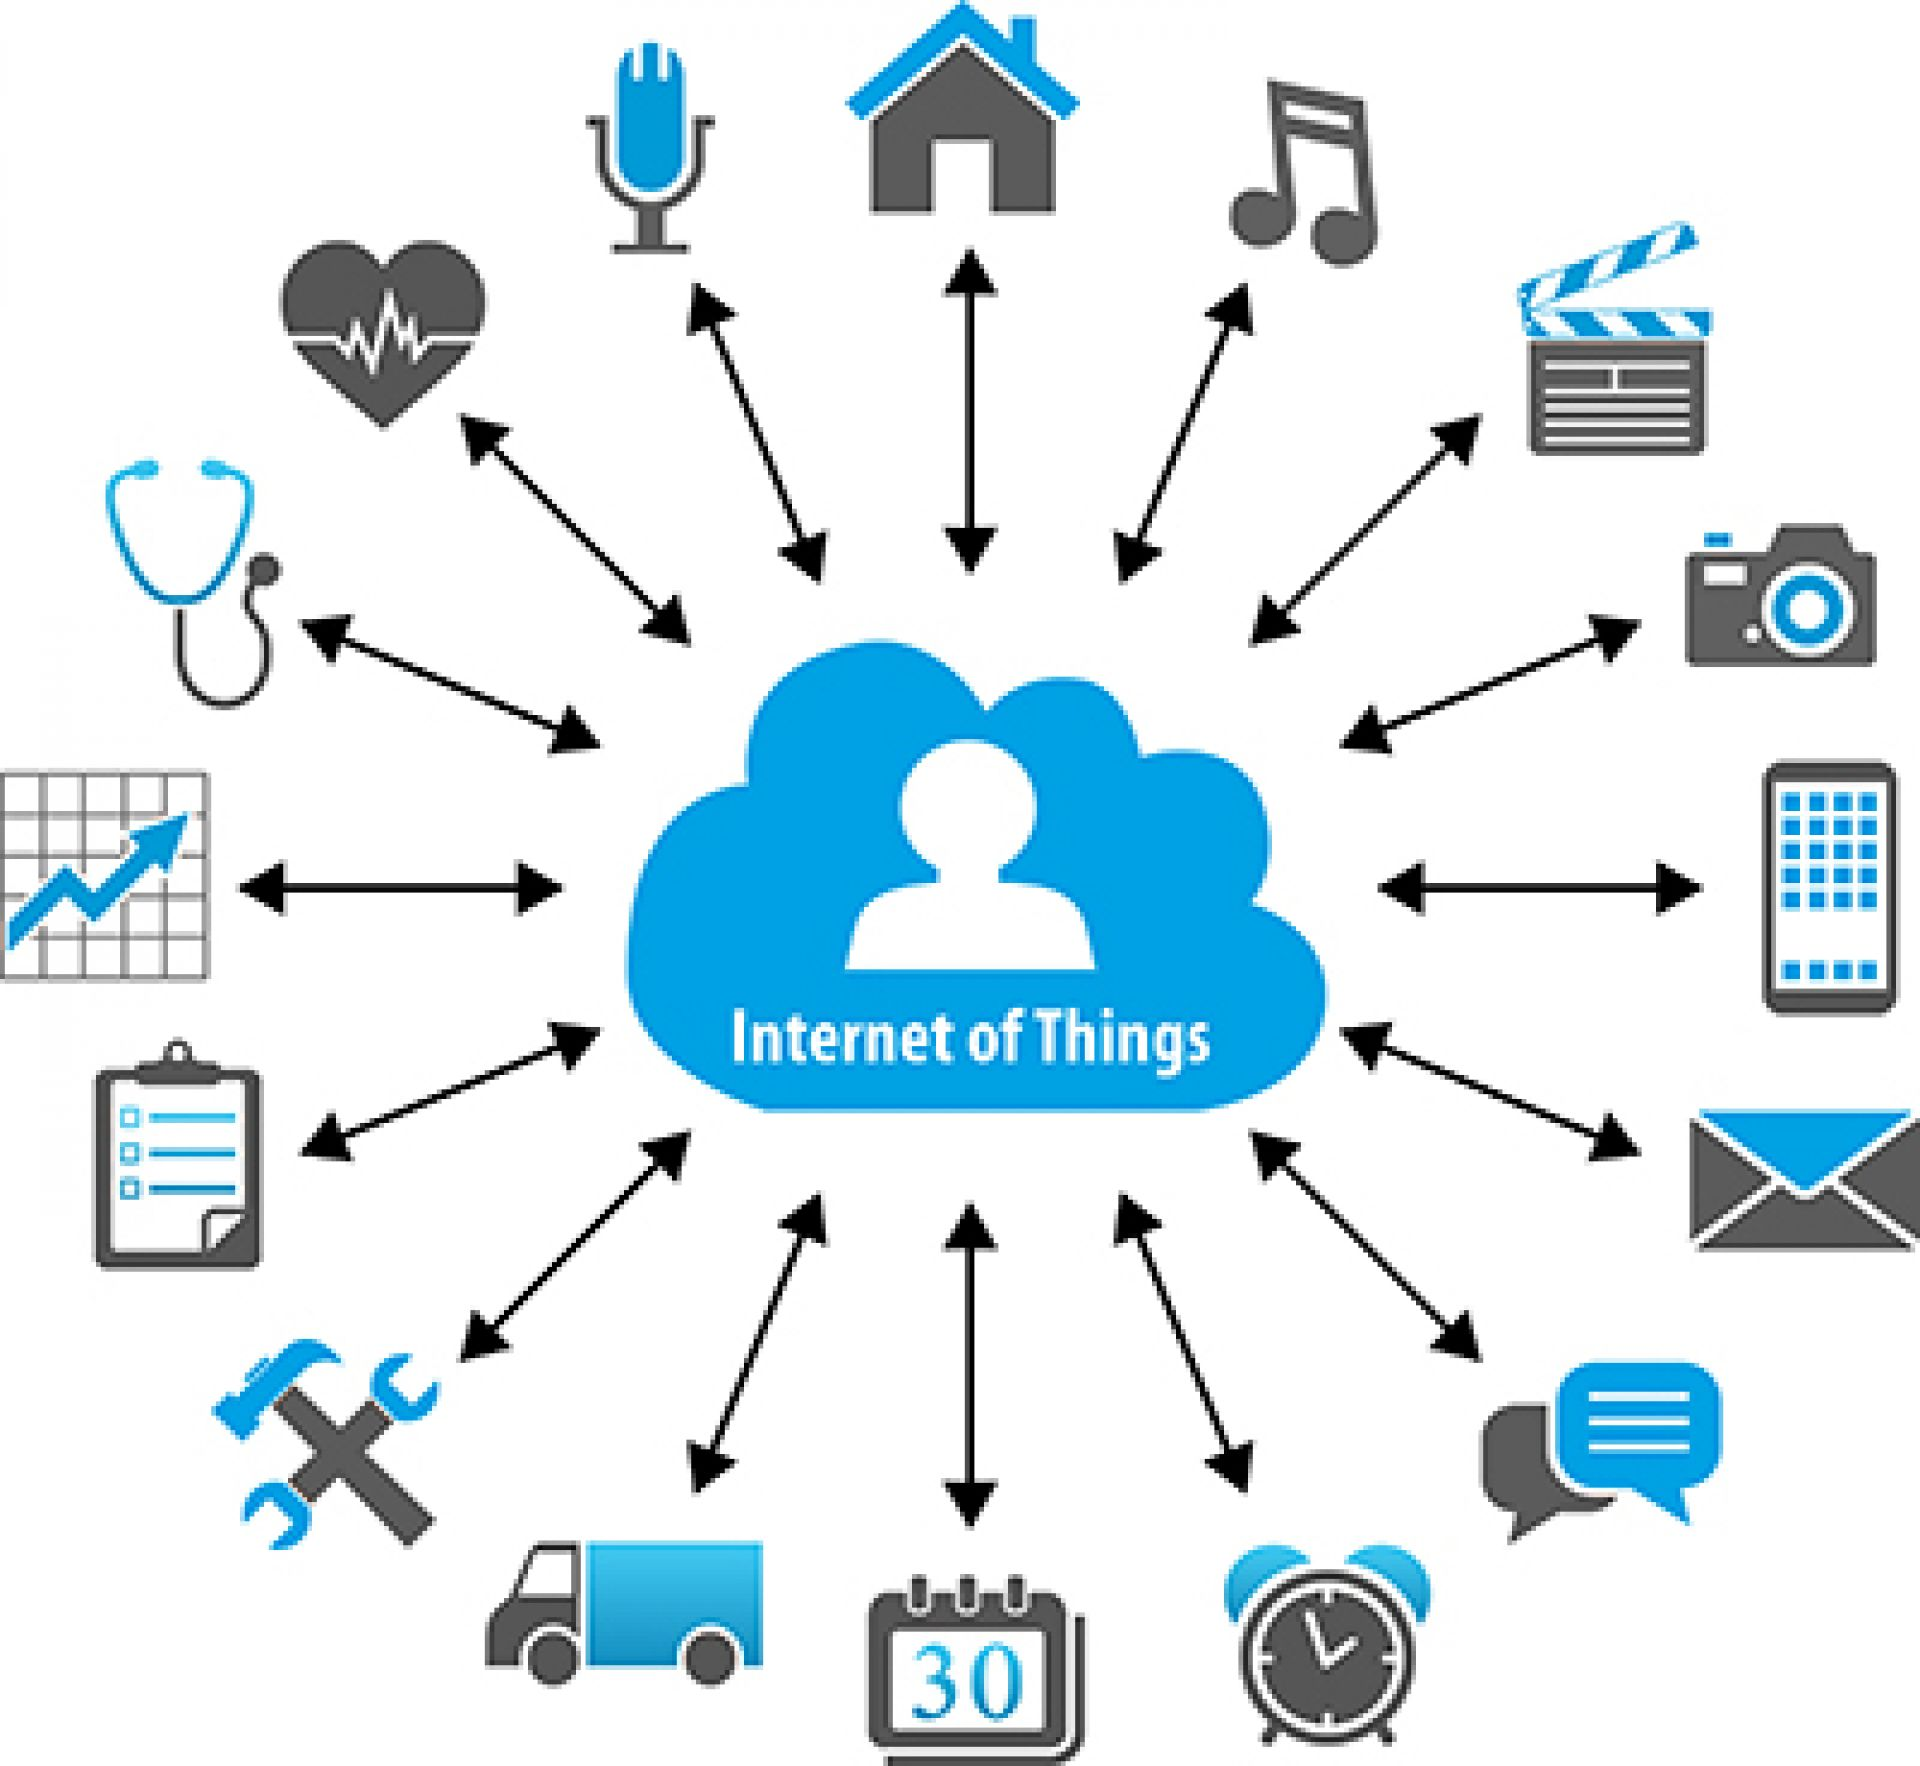
\includegraphics[height=1.75cm]{./images/Themes_IOT.jpg}}
%%%%%%%%%%%%%%%%%%%%%%%%%%%%%%%%%%%%%

%%%%%%%%%%%%%%%%%%%%%%%%%%%%%%%%%%%%%
\put(150,145){ \begin{minipage}[t]{0.75\linewidth}
{ \begin{itemize} \item Compte rendu de réunion \end{itemize} }
\end{minipage} }

\put(170,80){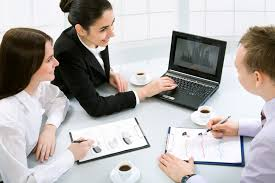
\includegraphics[height=1.75cm]{./images/Themes_meetings.jpeg}}
%%%%%%%%%%%%%%%%%%%%%%%%%%%%%%%%%%%%%

%%%%%%%%%%%%%%%%%%%%%%%%%%%%%%%%%%%%%
\put(235,105){ \begin{minipage}[t]{0.75\linewidth}
{ \begin{itemize} \item Rec. parcour\\ professionnel\end{itemize} }
\end{minipage} }

\put(245,25){
\includegraphics[height=1.75cm]{./images/Themes_Brain.jpg}}
%%%%%%%%%%%%%%%%%%%%%%%%%%%%%%%%%%%%%


%\put(210,140){\includegraphics[height=1.5cm]{./figures/CIRCLE_PACKING.png}}
%\put(110,140){\includegraphics[height=1.5cm]{./figures/PORTFOLIO_OPTIMIZATION_bis.jpg}}
%\put(250,50){\includegraphics[height=2.2cm]{./figures/POOLING_PROBLEM.jpg}}
%\put(100,50){\includegraphics[height=1.5cm]{./figures/UNIT_COMMITMENT.jpg}}


\end{picture}


\end{frame}

%------------------------------------------------
\begin{frame}{Travaux effectués - Les Méthodes Élicitation}
\textbf{Contexte}: Prédire des informations incertains dans le modèle en interrogeant le décisionnaire de systèmes
\vspace{0.2cm}

\begin{center}
communication avec l’utilisateur $\leftrightarrows$ \framebox{MOMDP} $\leftrightarrows$ la politique $\pi$
\end{center}
\vspace{0.2cm}

\textbf{Plusieurs approches}:
\begin{itemize}
\item Une approche itérative basée sur une function de valeur en utilisent des méthodes de clustering
\item calculer un ensemble pareto frontier de politiques offline, et ensuit communiquer avec l’agent.
\end{itemize}

\textbf{Résultat}: Le modèle trouve la politique optimale avec les moins
nombre possibles de communications avec l’agent ou décideur de
systèmes [STAIRS 2016, IJCNN 2016]

\end{frame}

%------------------------------------------------
\begin{frame}{Travaux effectués - Les Méthodes Optimisation}

%\textbf{Contexte}:Soit les récompenses sont incertaines et limitées. Peut-on trouver une politique robuste par rapport aux informations données dans le modèle? 

\textbf{Approche d’optimisation}: Calculer la politique optimale avec la méthode de minimax regret quand on peut pas savoir plus sur des préférences des utilisateurs.

\vspace{0.2cm}

\begin{center}
	\framebox{Master Programme} \\
	\vspace{0.1cm}
	Informations (solutions)~~~~~ $\downarrow$ ~~~~~ $\uparrow$ feed-backs (coupes)\\
	\vspace{0.1cm}
	\framebox{Slave Programme} 

\end{center}

\vspace{0.2cm}

\textbf{Plusieurs approches}:
\begin{itemize}
\item \textbf{Un calcul heuristique pour minimax-regret}: Générer des contraintes du programme linéaire aléatoirement au lieu de résoudre le programme linéaire exact.
\item \textbf{Résultat}: La méthode heuristique est plus rapide et applicable sur les modèles de grande taille [IEEE-RIVF 2015]
\end{itemize}

\end{frame}

%------------------------------------------------
\begin{frame}{Travaux effectués - Les Méthodes Optimisation}

\begin{itemize}
\item \textbf{Calculer les politique déterministes}: proposer un branch-and-bound basé sur le Benders decomposition. %comme bounding procedure.
\item \textbf{Résultat} [soumis à ECML 2018]: 
	\begin{itemize}
	\item Dans un temps $8$ fois plus lent, on trouve la politique déterministe avec le regret 	$25 \%$ moins que la politique stochastique   
	\item Théocratiquement, on preuve que 
	$$\frac{\text{regret de politique stochastic}}{\text{regret de politique deterministe}} = 2 $$
	\end{itemize}
\end{itemize}

\end{frame}

%------------------------------------------------
\begin{frame}{Travaux effectués \\ Les Applications et les réseaux de neurones}

\begin{columns}
\begin{column}{0.6\textwidth}
   
	\textbf{Contexte}: Composition de web service\\
	\vspace{0.2cm}
	\textbf{Question}: Il faut sélectionner laquelle service dans chaque service abstract tel que: les qualités des services convient les préférences des utilisateurs%, Et minimiser l’énergie totale consommée par les services sélectionnés  
\\	
	\vspace{0.2cm}
	\textbf{Approche}: Modéliser la probleme comme une MDP avec des objectives de qualité de service et Implémenter l'algorithme d'ABVI.
\end{column}
\begin{column}{0.4\textwidth}  %%<--- here
    \begin{center}
     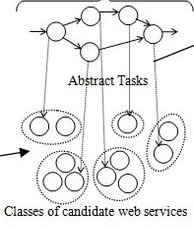
\includegraphics[width=0.8\textwidth]{images/web-service}
     \end{center}
\end{column}
\end{columns}

\end{frame}
%------------------------------------------------
\begin{frame}{Travaux effectués \\ Les Applications et les réseaux de neurones}
\textbf{Contexte}: Recherche des informations et entités nomes dans les documents en l'internet 
\begin{center}
 nom d'expert $\longrightarrow$ \framebox{Système} $\longrightarrow$ parcours professionnelle d'experte  
\end{center}
\textbf{Approche de RL profond}: Modéliser le problème comme une MDP et trouver le meilleurs parcours avec  algorithm de Deep Q-network. 

\textbf{Résultat}: On arrive à extraire le parcours professionnelle de chaque personne avec une bonne precision et en générant moins des requêtes sur le moteurs de recherche.  
\end{frame}
%------------------------------------------------
\begin{frame}{Travaux effectués - TAL \\ Compte rendu de Réunion}
\vspace{-0.5cm}
	\begin{center}
     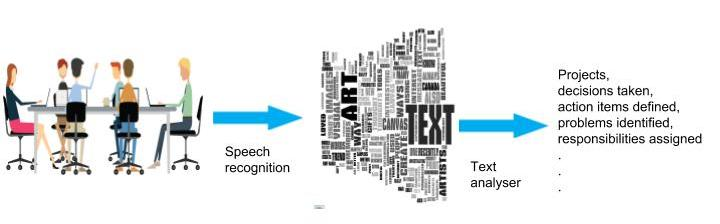
\includegraphics[width=0.7\textwidth]{images/reus-image} \\
	\end{center}
%

\textbf{Contexte}: Extraire des informations importants et structurés de réunions comme le projet, décisions, problèmes lies a projets et etc. \\

\textbf{Plusieurs Approches}:
\begin{itemize}
	\item regroupement des réunions avec les méthodes topic modeling et tf-idf. 
	\item extraire des informations caractérisations de chaque réunions avec le tf-idf. 
	\item Identification des actes de dialogues avec les méthodes non-supervisées et apprentissage profond (comme LSTM)
\end{itemize}

\end{frame}

%------------------------------------------------
\begin{frame}{publications}
Articles acceptés:\\
\begin{itemize}

\item [1] Pegah Alizadeh, Peggy Cellier, Bruno Crémellieux, Thierry Charnois et Albrecht Zimmermann. An Experimental Approach For Information Extraction in Multi-Party Dialogue Discourse, \textbf{CICLING 2018}\\


\item [2] P. Alizadeh, Y. Chevaleyre et F. Lévy. Solving MDPs with Unknown Reward Using Nondominated Vector-Valued Functions. \textbf{ECAI (STAIRS) 2016}\\


\item [3] P. Alizadeh, Y. Chevaleyre et F. Lévy. Advantage Based Value Iteration for Markov Decision Processes with Unknown Rewards.\textbf{IJCNN 2016}\\

\item [4] P. Alizadeh, Y. Chevaleyre et J. D. Zucker. Approximate regret based elicitation in Markov Decision Process. \textbf{IEEE-RIVF 2015} \\

\end{itemize}

\end{frame}
%------------------------------------------------
\begin{frame}{publications}

Articles soumis:\\

\begin{itemize}
	\item Pegah Alizadeh, Emiliano Traversi et Aomar Osmani. Deterministic Solutions Based on Maximum Regrets in Markov Decision Processes with Imprecise Rewards. %, \textbf{ECML 2018}
	\item Pegah Alizadeh, Aomar Osmani, Abdelghani Chibani, Yacine Amirat et Mohamed Essaid Khanouche. Interactive QoS-aware Services Selection for the Internet of Things.
\end{itemize}

Articles en préparation:\\
\begin{itemize}
	\item Pegah Alizadeh, Peggy Cellier, Bruno Crémellieux, Thierry Charnois et Albrecht Zimmermann. An Unsupervised Learning Approach for Dialogue Act Tagging in Multi-Party Dialogues. 
\end{itemize}

\end{frame}

%------------------------------------------------
%------------------------------------------------
\begin{frame}{Projet d'Intégration}

\end{frame}


%------------------------------------------------

\setbeamercolor{background canvas}{bg=blue!20}
\begin{frame}
	\begin{center}
	\textbf{Enseignement}
	\end{center}
\end{frame}
{\setbeamercolor{background canvas}{bg=white}

%-----------------------------------------------
\begin{frame}{Avant, Durant et Après la Thèse}
\begin{block}{Avant la Thèse (2,5 ans aux universités en Iran)}
Différents cours en \textbf{mathématique et statistique} aux étudiants de licence et ingénierie en informatique, statistique et économie.
\begin{itemize}
\item Precalculus, Calculus I, Calculus II. Equations Différentielles Ordinaires. Statistiques. Algèbre Linéaire Numérique.
\end{itemize}
\end{block}

\begin{block}{Durant la thèse (2 ans Monitrice -- 128 heurs)}
Des étudiants de 1ère et 2ème année en \textbf{Informatique à l'IUT} de Paris 13.

\begin{itemize}
\item Programmation (C++). Programmation et administration des BDD (Postgresql). Introduction aux interfaces homme- machine (Java,swing).
\end{itemize}
\end{block}

\end{frame}

%------------------------------------------------
\begin{frame}{Avant, Durant et Après la Thèse}

\begin{block}{Pendent la dernière année de thèse (192 heurs)}
Pour des élèves de \textbf{licence et master} en \textbf{Informatique} et \textbf{économie} à l'Institut Galilée de \textbf{Paris 13}.
\begin{itemize}
 \item Administrateur système (Marionnet), Unix
 \item Élément Informatique, Programmation impérative, Interface graphique (C, GTK)
 \item Bases de données, Bases de données avancées (Oracle)
\end{itemize}
\end{block}
%%%%%
\begin{block}{Demi ATER (100 heurs)}
j'ai enseigné à l'université \textbf{Paris Dauphine} aux étudiants de licence en \textbf{mathématique, informatique et économie}.
\begin{itemize} 
\item Programmation objet et objet avancée (Java)
\item Visual Basic Applications (responsable du cours)
\end{itemize}

\end{block}
\end{frame}
%------------------------------------------------
\begin{frame}{Encadrement de Projet}
J'ai encadré des comme vacation à université de Caen Normandie. 
\begin{block}{Projet de Master2}
\begin{itemize}
 \item Implémentation de Deep Q-network : le trading des cryptomonnaies
 \item Génération du texte avec une méthode de Deep Learning (LSTM)
\end{itemize}
\end{block}

\begin{block}{Stage de Licence 3}
\begin{itemize}
	\item
	\item 
\end{itemize}
\end{block}

\end{frame}

%-----------------------------------------------
\begin{frame}{Projet d’enseignement}

\end{frame}
%------------------------------------------------
\begin{frame}
\frametitle{References}
\footnotesize{
\begin{thebibliography}{99} 

\bibitem[Narasimhan et al., 2016]{Narasimhan}Karthik Narasimhan, Adam Yala and Regina Barzilay. (2016)
\newblock Improving Information Extraction by Acquiring External Evidence with
Reinforcement Learning. 
\newblock \emph{EMNLP}
%%
\bibitem[Benavent et Zanuttini, 2017]{Kim2015} Florian Benavent and Bruno Zanuttini. (2017)
\newblock An Experimental Study of Advice in Sequential Decision-Making under
Uncertainty
\newblock \emph{AAAI}
%%
\bibitem[Kim et al.2016]{Kim2016} Weng, P., and Zanuttini, B.(2013)
\newblock Interactive value iteration for Markov decision processes with unknown rewards.
\newblock \emph{23rd International Joint Conference on Artificial Intelligence (IJCAI 2013)}
%%

%\bibitem[]{}
%\newblock
%\newblock \emph{}
\end{thebibliography}
}
\end{frame}

\end{document} 
